\section{Data}
\label{sec:data}

\subsection{Surveys:  KiDS, BOSS and 2dFLenS}
\label{sec:surveys}

The Kilo-Degree Survey \citep[KiDS,][]{dejong/etal:2013}, spans 1350 sq degrees split into two fields, one
equatorial and one southern.    Matched-depth imaging in nine bands spans the optical,
$urgi$, through to the near-infra-red, $ZYJHK_s$, where the
near-infra-red imaging was taken as part of the KiDS partner survey
VIKING \citep[the VISTA Kilo-degree INfrared Galaxy
survey,][]{edge/etal:2013}.  High quality seeing was
routinely allocated to the primary KiDS $r$-band VST-OmegaCAM observations, resulting in a
mean $r$-band seeing of 0.7 arcseconds, with a maximum of 0.8
arcseconds.  This combination of full-area spatial and wavelength
resolution over a thousand square degrees,
provides a unique weak lensing survey that allows for enhanced
control of systematic errors \citep{giblin/etal:inprep, hildebrandt/etal:inprep}.
This analysis uses data from the fourth KiDS
data release of 1006 square degrees of imaging, (hence the name KiDS-1000), which has an effective
area, after masking, of 777 square degrees.  KiDS is a public survey from the European Southern
Observatory, with data products freely accessible through the ESO
archive\footnote{KiDS data access: \href{http://kids.strw.leidenuniv.nl/DR4}{kids.strw.leidenuniv.nl/DR4}}.   

The Baryon Oscillation Spectroscopic Survey
\citep[BOSS,][]{alam/etal:2015}, spans an effective area of 9329 square
degrees, with spectroscopic redshifts for 1.2 million luminous red
galaxies (LRG) in the redshift range $0.2<z<0.9$.   A range of
different statistical analyses of the clustering of BOSS galaxies have been used in combination with CMB
measurements, to set tight contraints on extensions to the standard
flat $\Lambda$CDM model \citep[see][and references
therein]{alam/etal:2017}.   We adopt the anisotropic clustering
measurements of \citet{sanchez/etal:2017} in this multi-probe analysis.
BOSS only overlaps with the equatorial stripe
of the KiDS survey, with 409 square degrees of the BOSS survey lying within
the KiDS-1000 footprint.  BOSS galaxies in this overlapping region are used as lenses in
our galaxy-galaxy lensing analysis, with an effective lens number density of 0.031
galaxies per square arcmin.  BOSS is a public survey from the third Sloan
Digital Sky Survey\footnote{BOSS data access: \href{https://data.sdss.org/sas/dr12/boss/lss/}{data.sdss.org/sas/dr12/boss/lss/}}.   

The two-degree Field Lensing Survey
\citep[2dFLenS,][]{blake/etal:2016}, spans 731 square degrees, with
spectroscopic redshifts for 70,000 galaxies out to $z<0.9$.   This
galaxy redshift survey from the Anglo-Australian Telescope was designed
to target areas already mapped by weak lensing surveys to facilitate `same-sky'
lensing-clustering analyses
\citep{johnson/etal:2017,amon/etal:2018,joudaki/etal:2018}.
We use data from the 2dFLenS LRG sample that was targetted to match
the BOSS-LRG selection, but with sparser sampling.  2dFLenS
thus provides an additional sample of BOSS-like galaxies in the KiDS
southern stripe where there is 425 square degrees of overlap within
the KiDS-1000 footprint.  2dFLenS galaxies in this overlapping region are used as lenses in
our galaxy-galaxy lensing analysis, with an effective lens number density of 0.012
galaxies per square arcmin.  2dFLenS is a public survey\footnote{2dFLenS data
  access: \href{http://2dflens.swin.edu.au/data.html}{2dflens.swin.edu.au/data.html}}.   




\subsection{Cosmic Shear}
\label{sec:cosmic_shear}
The KiDS-1000 cosmic shear power spectra from \citet{asgari/etal:inprep} is shown in Figure~\ref{fig:Pkk}.

\begin{figure*}
        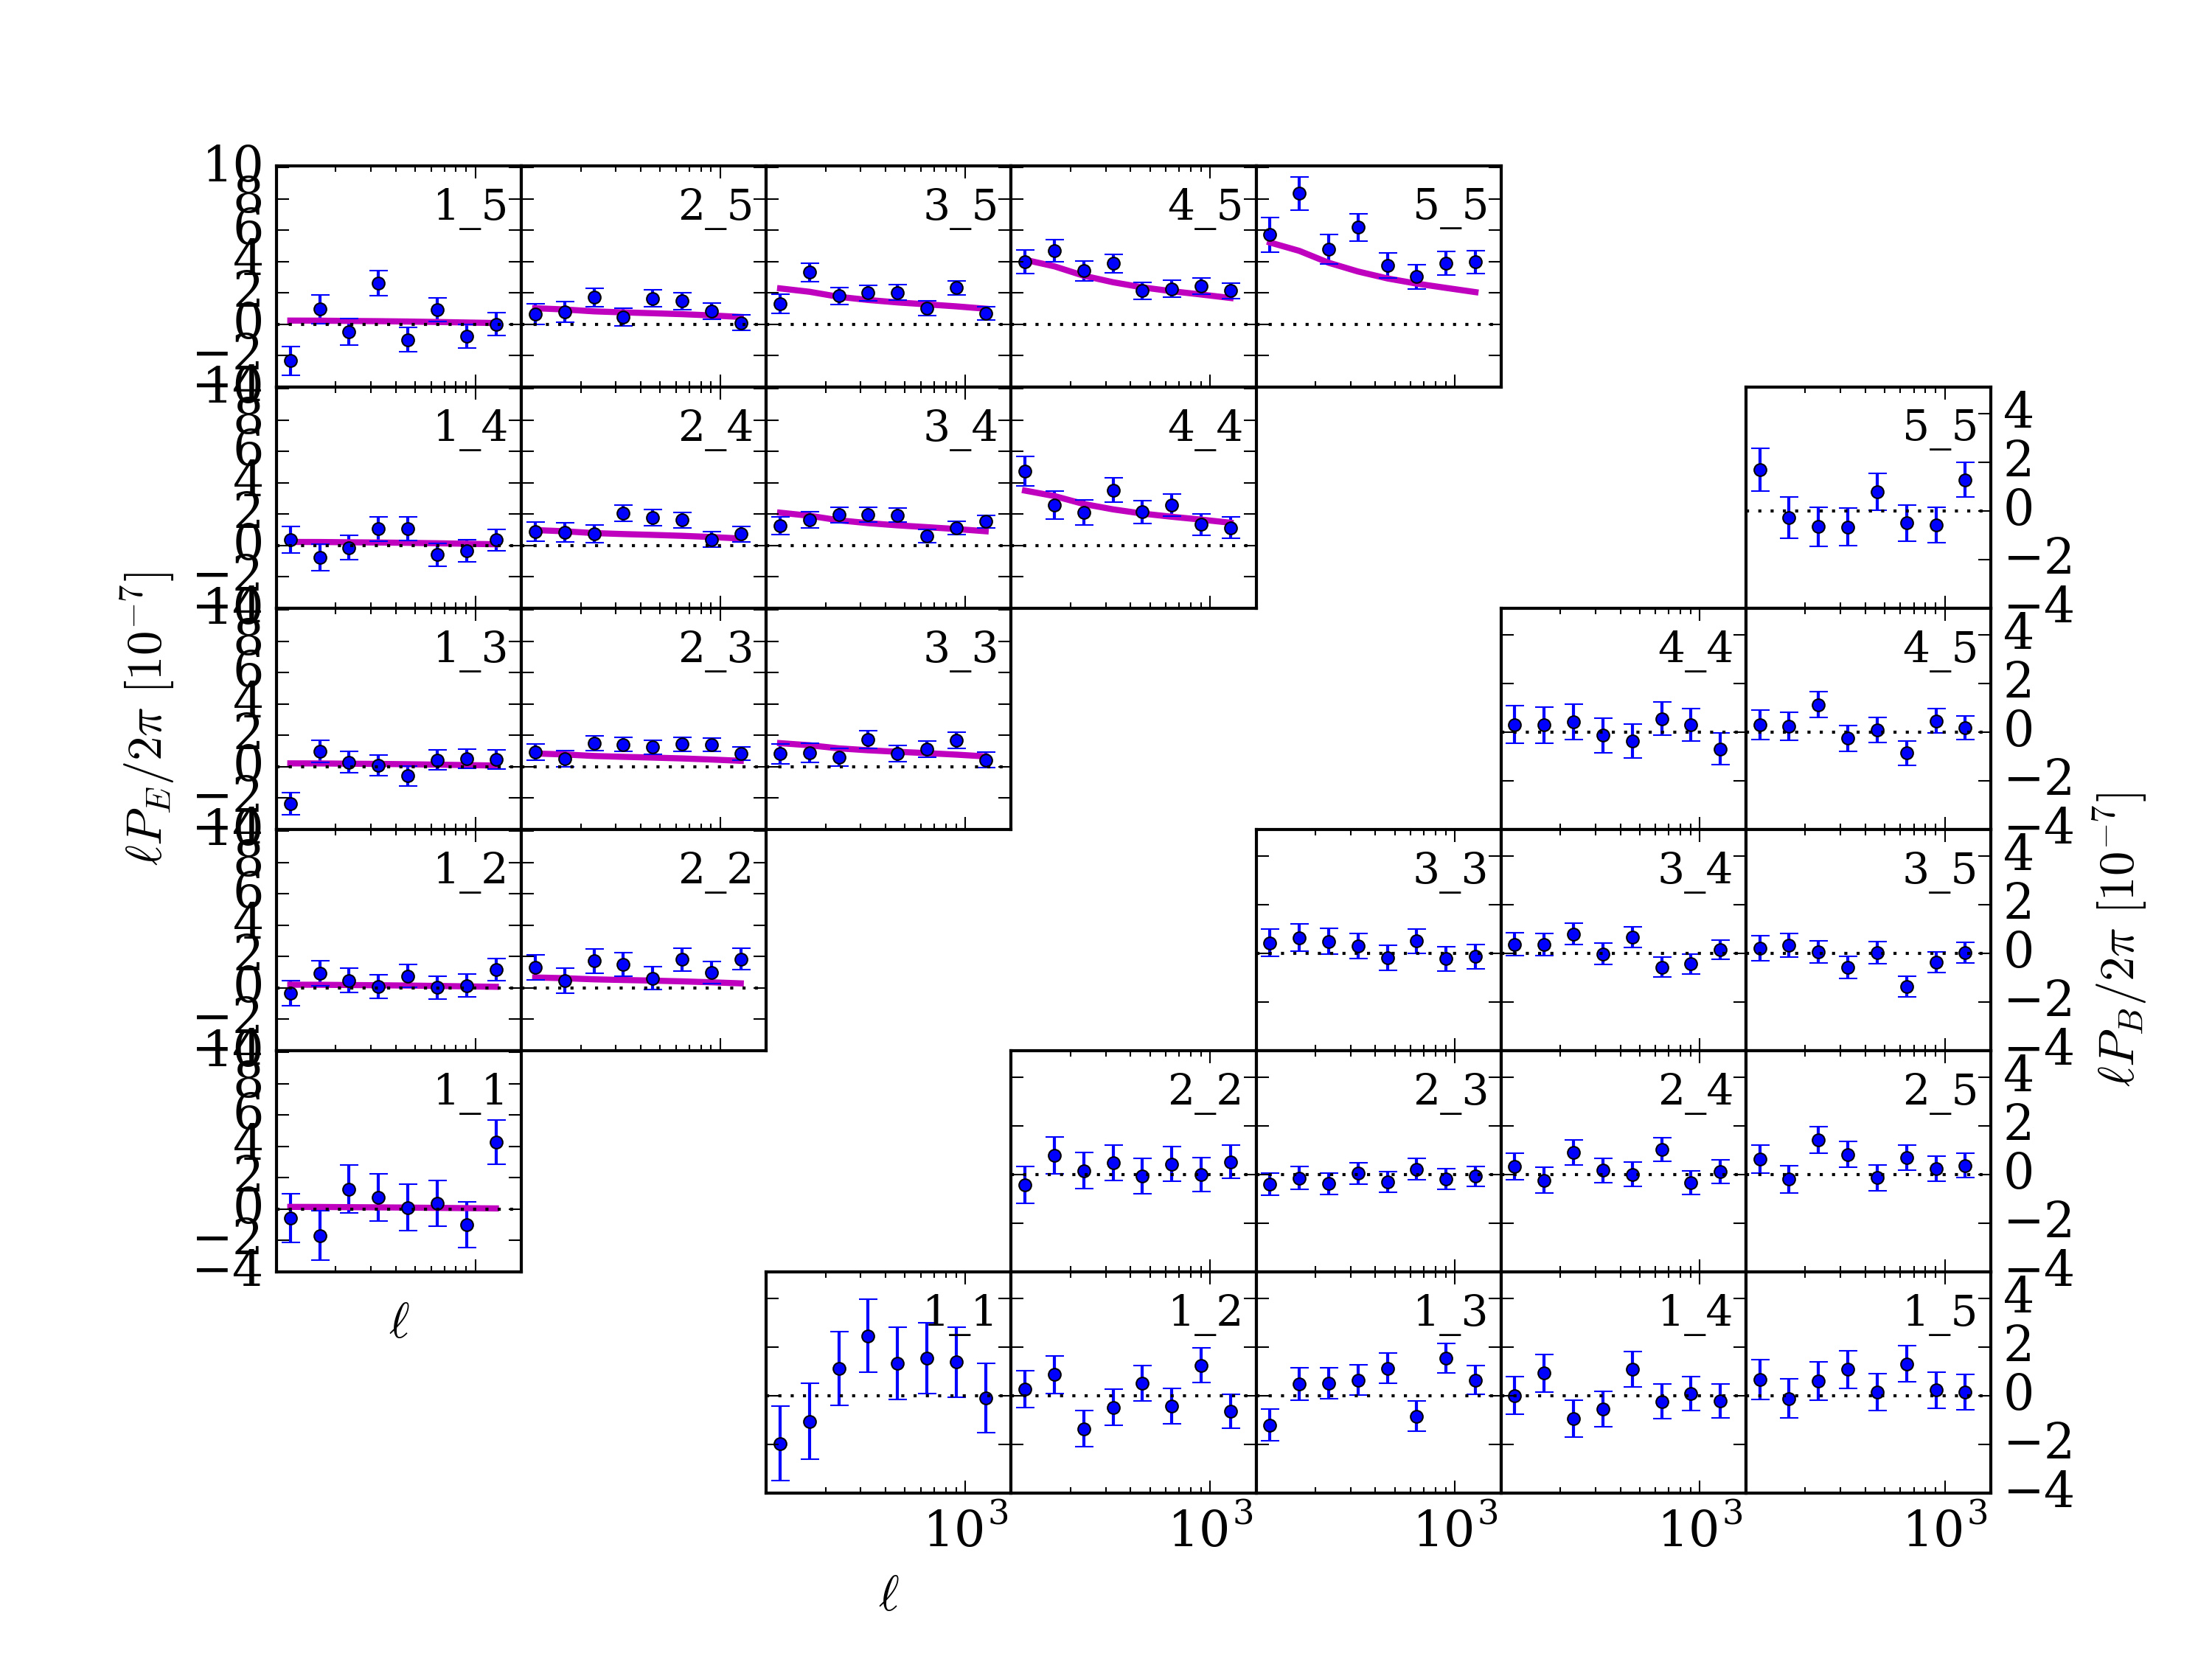
\includegraphics[width=\textwidth]{Data_Plots/Pkk/Pkk_K1000_2Dbins_v2_goldclasses_Flag_SOM_Fid.png}
        \caption{KiDS-1000 cosmic shear power spectra:  Tomographic
          band powers comparing the E-modes (upper left block) with the best-fit
          cosmological model from our combined multi-probe analysis
          \ch{TO DO}.  The tomographic
        bin combination is indicated in the upper right corner of each
      sub-panel.  The null-test B-modes (lower right block), are
      consistent with zero for both the full data vector, and each
     bin combination individually.}
        \label{fig:Pkk}
\end{figure*}

\subsection{Galaxy-Galaxy Lensing}
\label{sec:GGL}
Summary of Blake et al?


In Figure~\ref{fig:Pgk} we present the KiDS-1000 galaxy-galaxy lensing
power spectra, around lenses from the BOSS and 2dFLenS surveys.

\begin{figure*}
        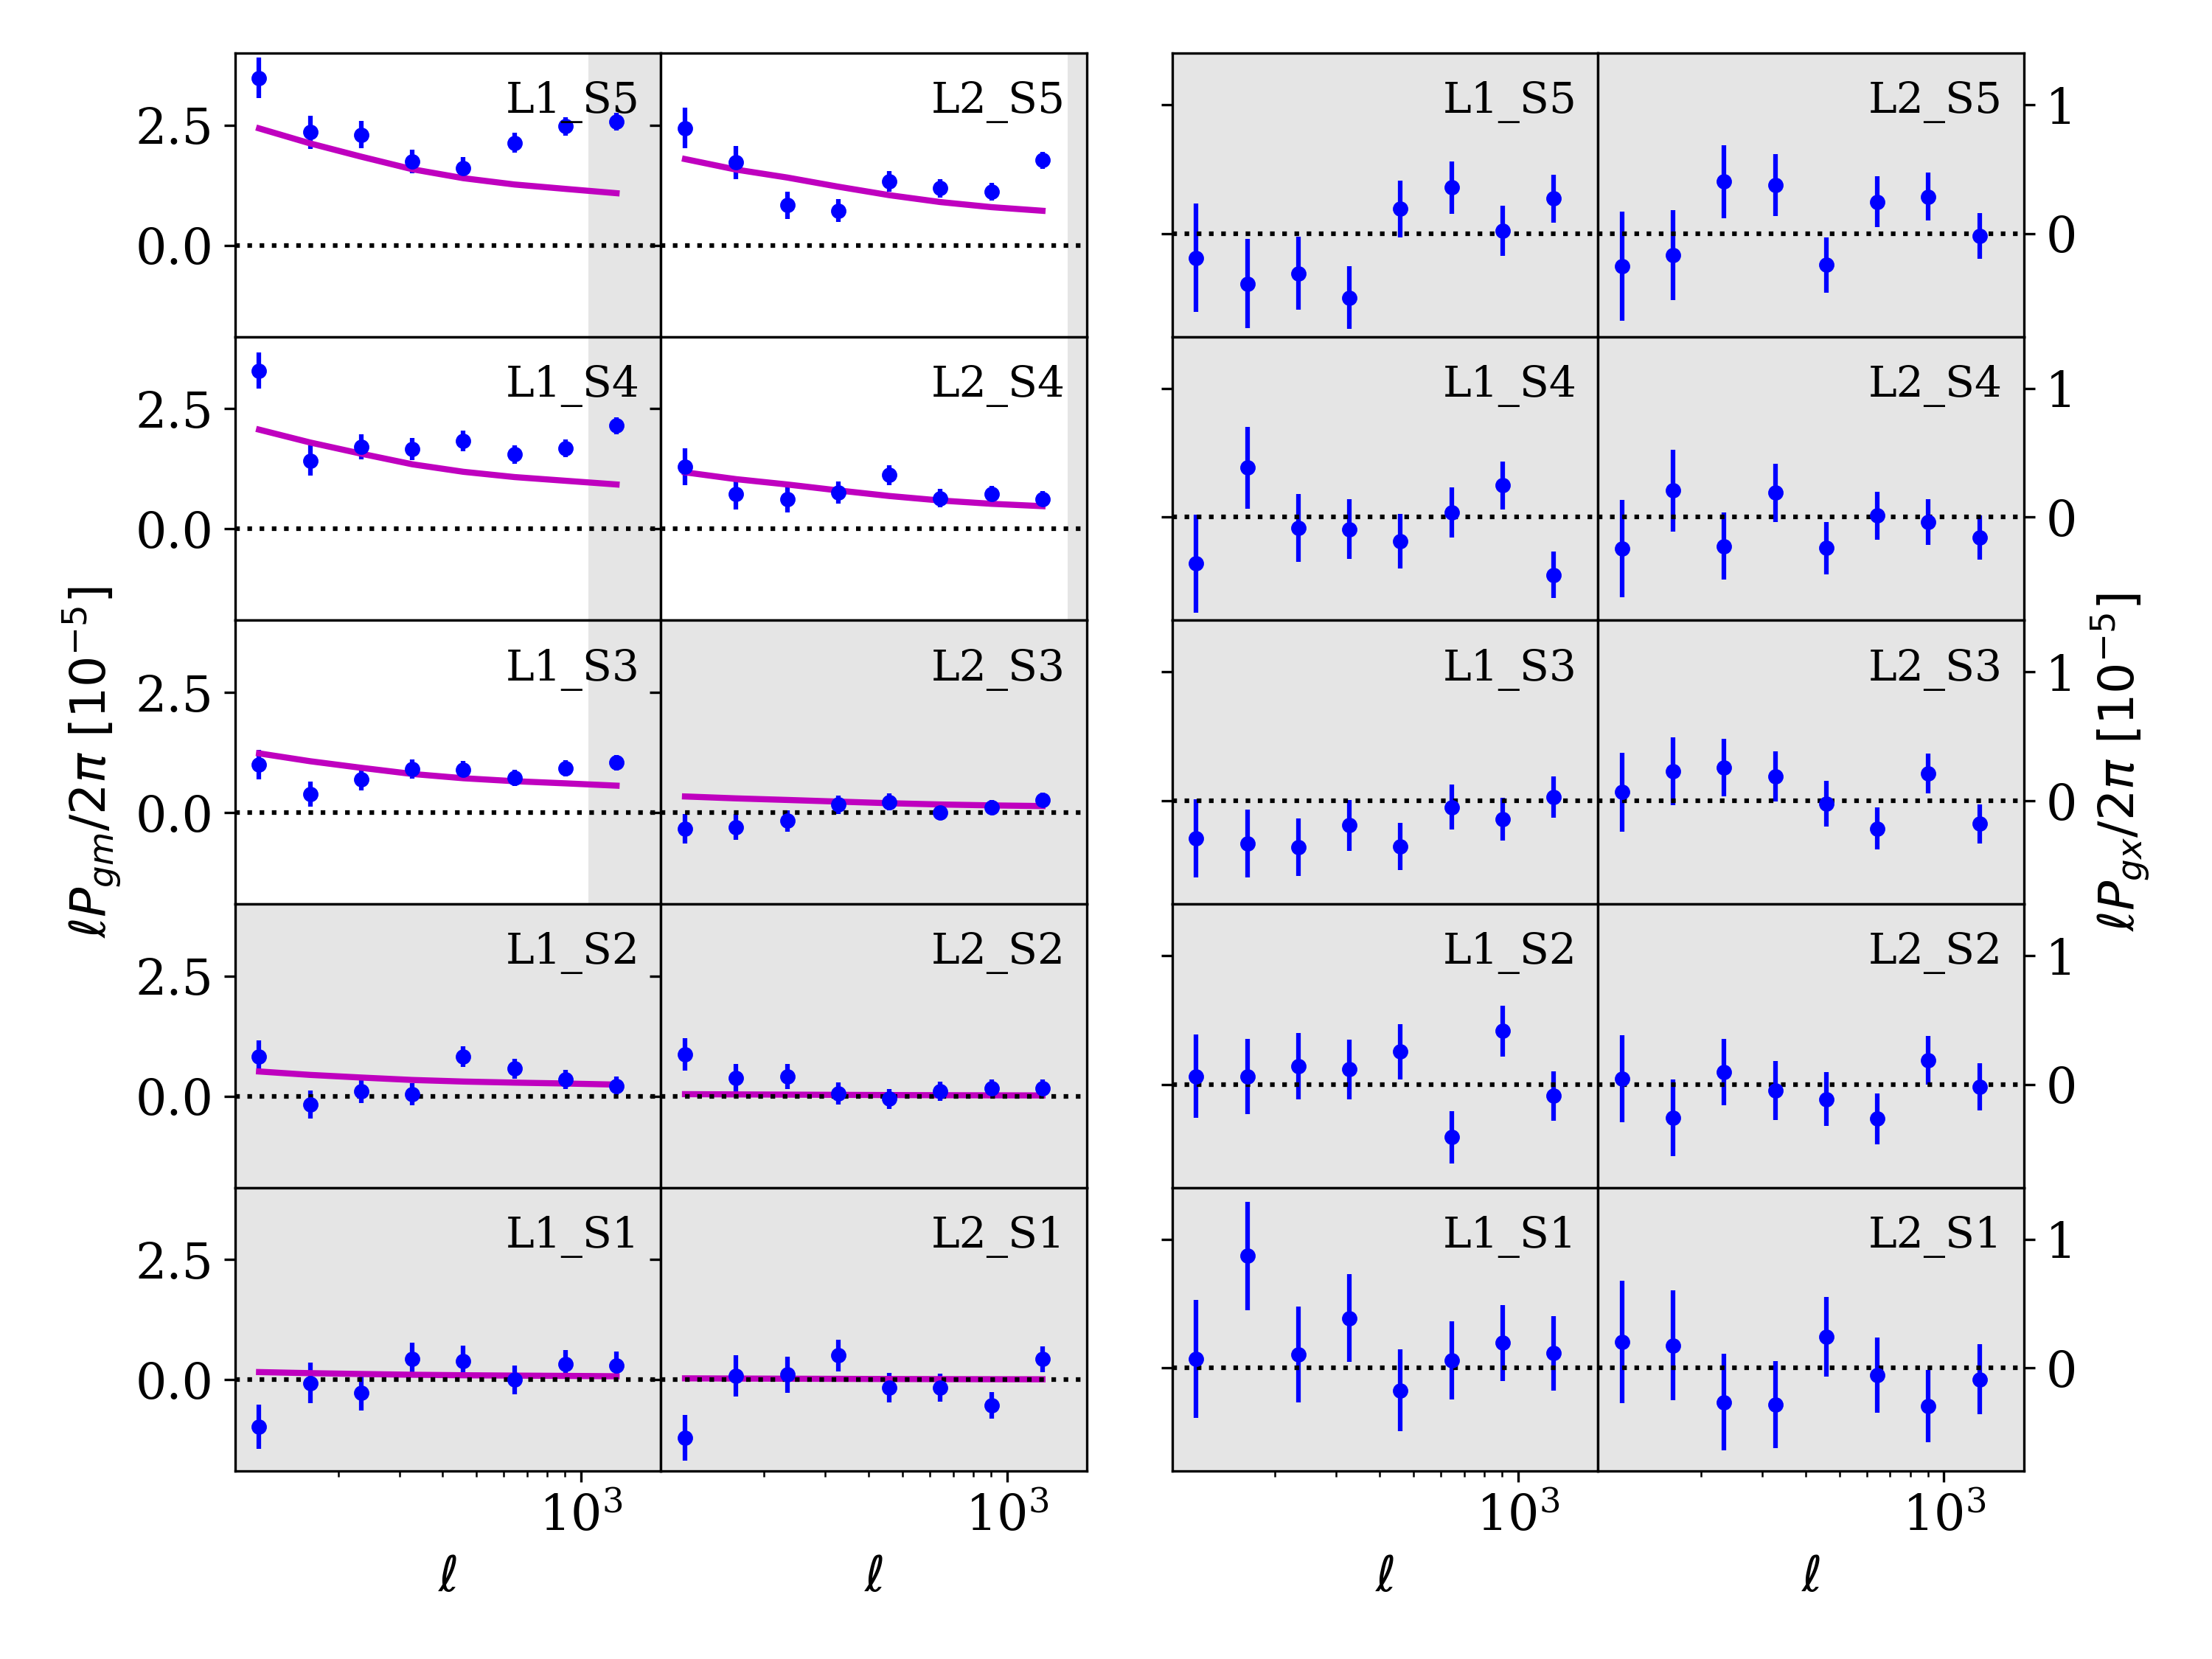
\includegraphics[width=\textwidth]{Data_Plots/Pgk/Pgk_K1000_2Dbins_v2_goldclasses_Flag_SOM_Fid.png}
        \caption{KiDS-1000 galaxy-galaxy lensing power spectra:
          Tomographic band powers comparing the E-modes (left block)
          with the best-fit
          cosmological model from our combined multi-probe analysis
          \ch{TO DO}.  The tomographic 
        bin combination of BOSS and 2dFLenS lenses (L) with KiDS-1000
        sources (S), is indicated in the upper right corner of each
        sub-panel.  Data within grey-regions are not included in the cosmological analysis.
        The null-test B-modes (right block), are
      consistent with zero for both the full data vector, and each
     bin combination individually \ch{TO DO}.}
        \label{fig:Pgk}
\end{figure*}

\subsection{Anisotropic Galaxy Clustering}
\label{sec:clustering}
Summary of \citet{sanchez/etal:2017}

In Figure~\ref{fig:wedges} we present the BOSS-DR12 anisotropic
clustering wedges.
\begin{figure*}
        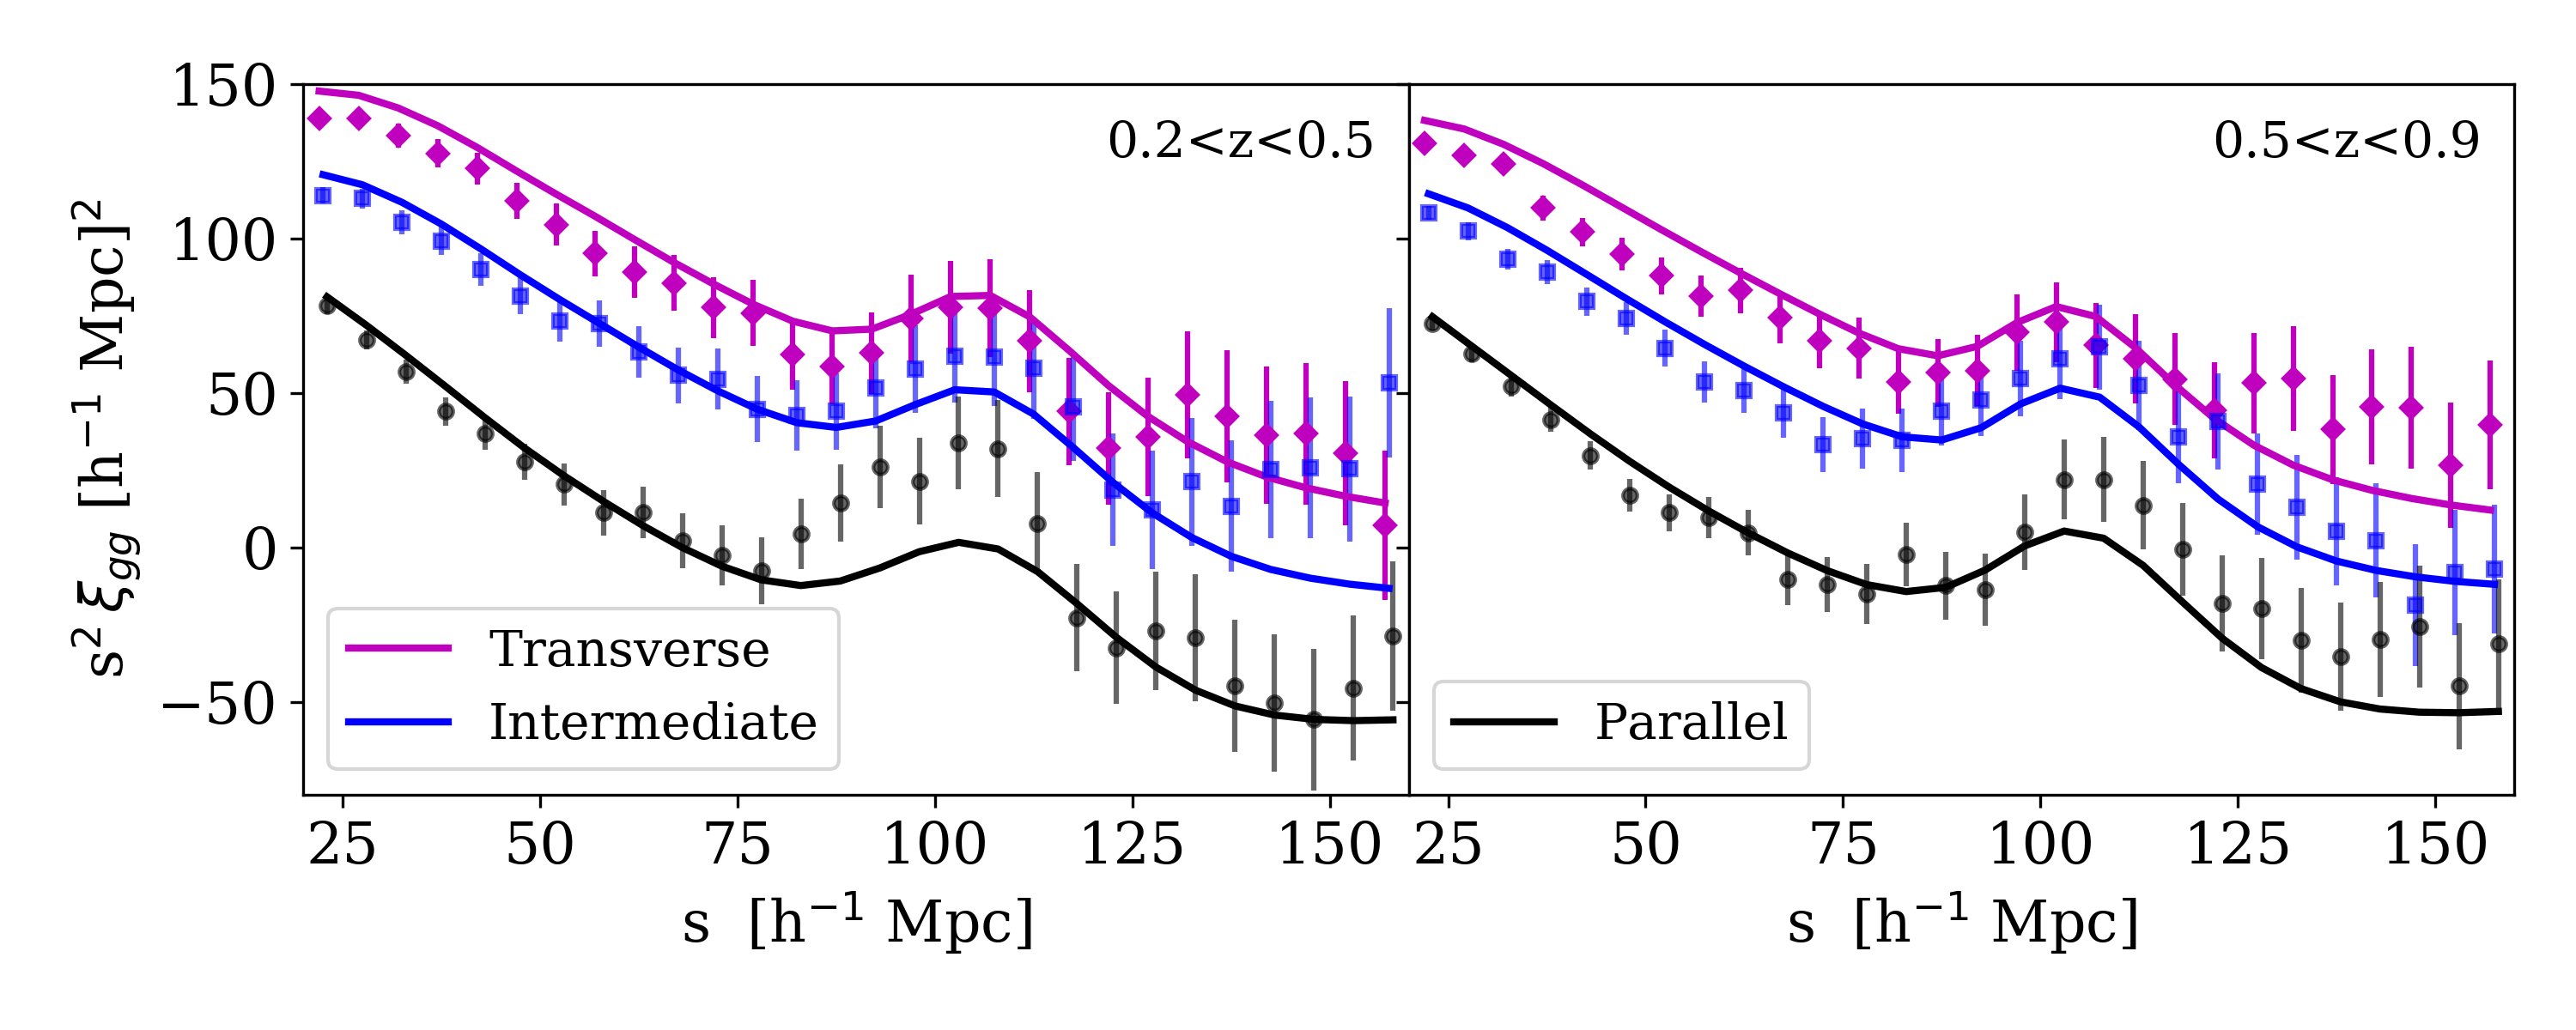
\includegraphics[width=\textwidth]{Data_Plots/clustering_wedges/BOSS_Sanchez_wedges.png}
        \caption{BOSS-DR12 anisotropic clustering from \citet{sanchez/etal:2017}:
          The transverse (pink), intermediate (blue) and parrallel
          (black) clustering wedges in two redshift bins, compared 
          with the best-fit
          cosmological model from our combined multi-probe analysis
          \ch{TO DO}.}
        \label{fig:wedges}
\end{figure*}

\subsection{Covariance}
\label{sec:Cov}
Summary of \citet{joachimi/etal:inprep}

